\chapter{Overview}
\label{sct:overview}

The job execution in Grid infrastructures of LHC experiments is done using so-called \indexed{pilot job} approach: experiments come into posession 
of Grid resrouces using special kind of jobs, known as '\indexed{pilot job}s' (or 'job agents', 'pilot agents', 'pilots'), after which they use their 
own job submission and scheduling systems (e.g. \cite{alien, dirac, panda, crab} ) to deliver and execute Grid users' jobs on those resources. 

After landing on the worker nodes of the computing sites the \indexed{pilot job}s inspect the machine configuration (e.g. check which software packages 
are available), make necessary preparations for the execution of the real job (e.g. install experiment application packages), report to the experiment 
scheduling system the configuration of the machine (e.g. available disk space and memory), fetch the real job for execution, fork a process and start 
execution of the real job within that process. 

\cernvmcopilot\ is a framework for execution of LHC experiments' \indexed{pilot job}s on a wide choice of extra (and so far untapped by 
LHC experiments) computing resources such as enterprise cloud computing infrastructures (e.g. Amazon EC2 \cite{ec2}), scientific computing 
clouds (e.g. Nimbus \cite{nimbus, scienceClouds} ), and, last but not least, cloud of BOINC (\cite{boinc}) volunteer PC's. \copilot\ serves 
as a gateway between differing \indexed{pilot job} implementations of the LHC experiments and cloud resources. On each experiment's side of 
the gateway so-called \copilot\ Adapter service is required. Currently such adapers have been developed for both ALICE and ATLAS, adapters 
for CMS and LHCb should be produced in order to complete the system.

In order to provide additional computing resources to the LHC experiments, it is important not to expect the physicists who run job production to 
make changes to their existing scripts or procedures, that is why the \copilot\ is designed in a way that the integration of the external 
resources is completely transparent for end-users.

All the code needed to support the \copilot\ services and to communicate with the Grid services of experiments is included in 
the \cernvm\ \cite{cernvm08, cernvmWeb} images that we use. The images also contain the ready-to-use LHC experiments' 
application frameworks.

The \copilot\ framework (Figure~\ref{fig:architecture}) consists of the \indexed{\copilot\ Agent} � a lightweight program which runs inside virtual 
machines deployed on the cloud, and of \indexed{\copilot\ Service}s -- components which orchestrate the work of \copilot
\ Agents. Agents and Services communicate by means of Jabber/XMPP \cite{rfc3920,rfc3921} instant messaging network using a 
specially developed protocol. The \copilot\ Service components are stateless which in conjunction with the use of Jabber/XMPP allows 
to scale the system in case of high load by just deploying new Service instances and adding them to the existing messaging network .  

Co-Pilot framework has two goals. The first goal is to integrate cloud resources with the existing grid infrastructures by seamlessly extending experiment grid pilot job frameworks. The second goal is to provide a toolkit which can be used to quickly instantiate an ad-hoc distributed computing infrastructure on top of cloud resources. Such a need often arises within the relatively small experiments or research groups (e.g. NA61 experiment~\cite{laszlo2009na61}, CERN Theoretical Physics group) which do not have enough resources to deploy and maintain a grid infrastructure. 


\begin{figure}
	\begin{center}
		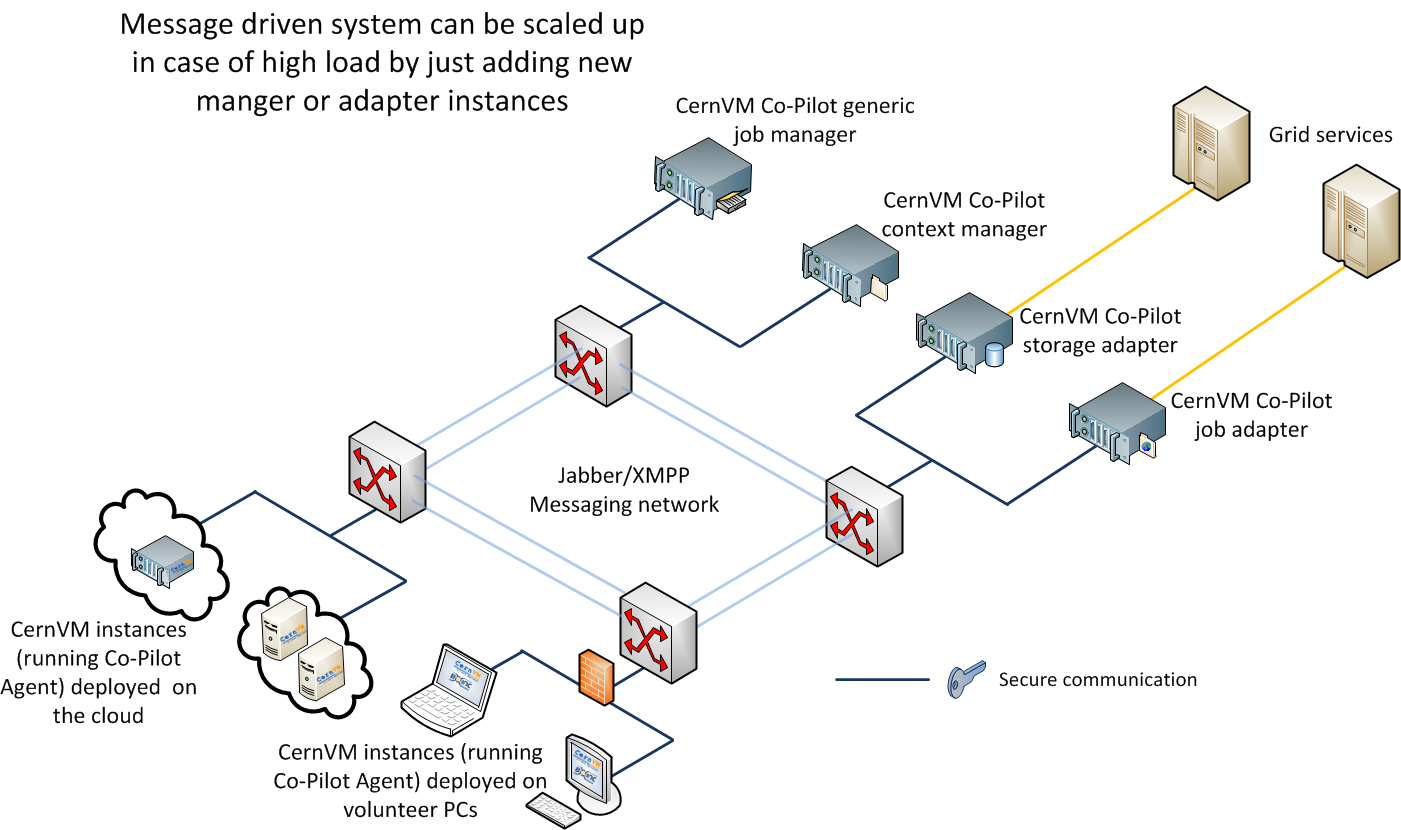
\includegraphics[scale=0.2]{img/IMG_Co-Pilot_Architecture.png}
	\end{center}
	\caption{The architecture of \cernvmcopilot framework}
	\label{fig:architecture}
\end{figure}

The components of the \copilot~framework are listed in Table~\ref{tbl:components}. 

\begin{table}
  \begin{center}

    \begin{tabularx}{\linewidth}{l|X}
      {\bf\centering \copilot component name} & {\bf\centering Description} \\\hline
        \texttt{Agent} & Communicates with service insances and requests a job to execute. Upon receiving the job downloads the input 
                         files, executes the job, uploads job output files and reports that the job execution is finished. \\
        \texttt{Generic Job and Storage Manager} & Distributes jobs from the internal queue to Agents for execution, provides space for storing 
                                                   the job output   \\
        \texttt{AliEn Job Manager} & Retrieves jobs from the central task queue of \indexed{AliEn} Grid \cite{alien} and sends them to 
                                     Agents for execution \\
        \texttt{AliEn Storage Manager} & Uploads the output of AliEn jobs executed by Agents and finalizes the job status in AliEn Grid.  \\
        \texttt{PanDA Storage Manager} & Uploads the output of \indexed{PanDA} \cite{panda} jobs executed by Agents and finalizes the job status in PanDA Grid  \\
    \end{tabularx}  
  \end{center}

  \caption{List of \copilot componentns}

  \label{tbl:components}
\end{table}


